\chapter{Oversikt over valgte Teknologier}
Dette kapittelet omfatter en oversikt over informasjon fra de valgte teknlogoier, og begrunnelser bak dette.tst
\section{Publisering}
Ett av kravene til prosjektet var at nettsiden skal være så selvstendig som mulig. Det skal være minimalt med nedetid, serveren må kunne oppdateres uten manuelt inngrep og backup av database må foregå automatisk. Samtidig som å oppfylle dette burde selve hostingen være så billig som mulig. Derfor ble det noe moderne konseptet av Platform as a Service benyttet.

\subsection{Platform as a Service}
En Platform as a Service (PaaS) er et utviklings og distribusjons miljø basert i en skytjeneste \cite{ paas:azure}. En PaaS leverandør har som ansvar å levere og opprettholde en utviklings og distribusjons plattform for sine kunder. De har videre ansvaret på områdene rundt konfigurering, oppsett av servere og sikkerhet på server siden. Det er populært å referere til  PaaS leverandører som IT-avdelingen til produktet, som gjør at utvikleren kan fokusere mer på selve utviklingen enn oppsett av infrastrukturen som ligger under \cite[s. 10]{bachelor}


\newpage
\section{Programmeringsspråk og Rammeverk}
Med dette prosjektet ville jeg videreutvikle min kompetanse innen bruken av rammeverket Django, basert på programmeringsspråket Python. 
\subsection{Python}
Python er et skriptingspråk utviklet av nederlandske Guide van Rossum. Den tidligste versjonen kom frem i 1996 og det har stadig vært i utvikling siden. Python har et formål om å gjøre kode leselig og gjenbrukbar, og har et mindre fokus på ren hastighet. Utover dette har Python et fokus på å gjøre utviklingen, og debuggings fasene av prosjekter så raskt som mulig \cite[s. 11]{bachelor}.
\subsection{Django}
Django er et web-applikasjons rammeverk som kommer levert med en ‘batterier inkuldert' filosofi. Dette betyr at vanlig funksjonalitet som ofte blir benyttet i en web sammenheng blir levert med i grunnpakken til Django. Dette inkluderer bruker-system, URL routing, template system, administrasjons system og database object-relational mapper (ORM) \cite{django:what}.



\begin{wrapfigure}{r}{4.5cm}
\caption[Django Oversikt]{Stegene Django kjører gjennom ved et HTML request. }\label{wrap-fig:1}
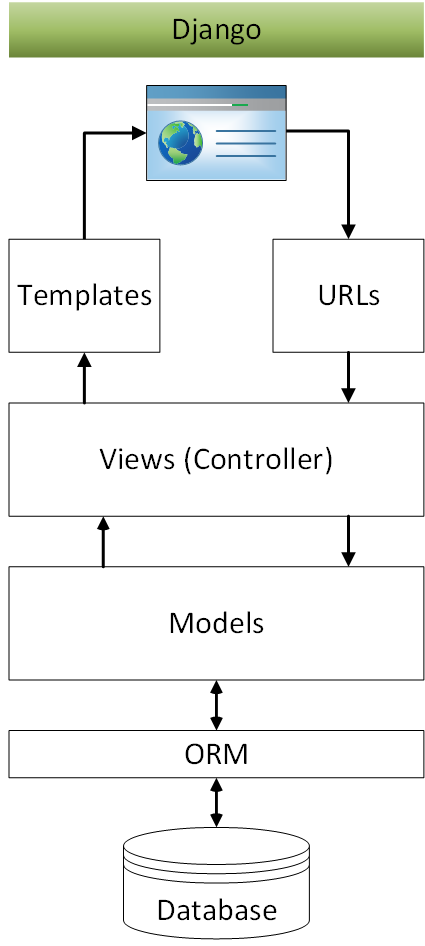
\includegraphics[width=4.5cm]{Bilder/django.png}
\end{wrapfigure}

På figur \ref{wrap-fig:1} kan man se en oversikt over hvordan Django håndterer et HTML request. 

Først vil den tyde hvilke URL som kommer inn. Django inneholder et register over tilgjengelige URL som kan benyttes vha. regular expressions. Den vil sjekke dette registeret og finne hvilken funksjon (view) som tilhører den innkommende URL.

Den korresponderende funksjon i view vil nå håndtere data fra HTML requestet, dette innebærer å sjekke om det er et POST eller GET request, og hente ut eventuell data med henyn til dette. 

Data vil bli hentet vha. Djangos Modeller, som er et objekt orientert metode å fremstille den tilkoblede databasen. Når det er klart hvilke data som skal hentes, vil Djangos ORM konvertere Djangos Database API til SQL Query. Den data som resulterer fra spørringen vil bli returnert tilbake til view.

Til slutt vil view samle data og generere den tilhørende template (html), som videre sendes tilbake til browseren.



\section{Frontend}
På klientsiden har det i hovedsak blitt benyttet 2 større 

